\documentclass[serif,usenames,dvipsnames,landscape]{beamer}
\usepackage[utf8x]{inputenc}
\usepackage{ucs}
\usepackage{amssymb}
\usepackage{amsmath}
\usepackage{gensymb}
\usepackage{amsfonts}
\usepackage{amssymb}
\usepackage{makeidx}
\usepackage{graphicx}
%\usepackage{kpfonts}
\usepackage{tikz}
\usepackage{xcolor}
\usetheme{Execushares}
\usecolortheme[named=NavyBlue]{structure}

%https://blog.hamaluik.ca/posts/better-beamer-themes/
%https://github.com/hamaluik/Beamer-Theme-Execushares
%https://nval.andreasherten.de/2016/09/13/beamer-tips.html
%https://tex.stackexchange.com/questions/116077/presentation-beamer-title-page

\author{Nicolás Espinoza Muñoz}
\title{MODELACIÓN NUMÉRICA DE UNA PROTEÍNA INSERTA EN UNA MEMBRANA CELULAR USANDO EL MÉTODO DE ELEMENTOS DE BORDE.}
\institute{UNIVERSIDAD TÉCNICA FEDERICO SANTA MARÍA}
\date{\today}

\begin{document}
	\maketitle
	\section{Motivación}
	
\begin{frame}{La célula}
	\begin{figure}
		\begin{minipage}{0.5\slidewidth}
			\begin{itemize}
				\item[$\bullet$] La membrana se encuentra en todas las células.
				\item[$\bullet$] Se compone de una doble capa de fosfolípidos.
				\item[$\bullet$] Tiene proteínas insertas.
			\end{itemize}
		\end{minipage}
	\vspace{15pt}
		\begin{minipage}{0.1\slidewidth}
			\hspace*{0.5cm}
		\end{minipage}%
%	\vspace{15pt}
		\begin{minipage}{0.2\slidewidth}
			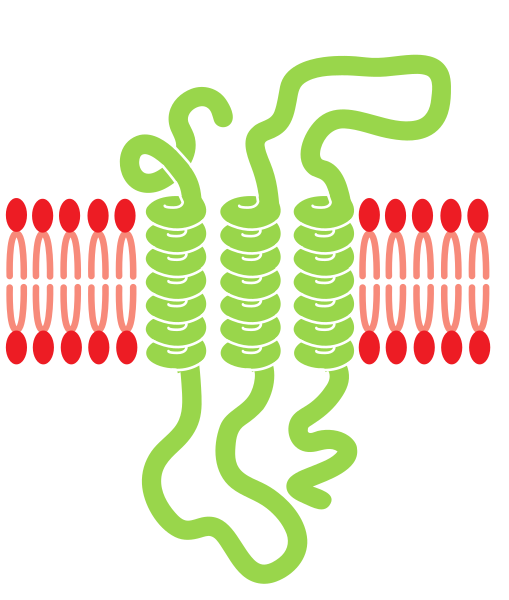
\includegraphics[scale = 0.15]{./Figures/Alberts_mem_protein.png}
		\end{minipage}
	\vspace{-50pt}
		\begin{minipage}{0.45\slidewidth}
			\input{./Figures/Fig_5-2.eps_tex}
		\end{minipage}
	\end{figure}
\end{frame}

\begin{frame}{Representaciones}
	\begin{figure}
		\begin{minipage}{0.34\slidewidth}
			{\Large \textbf{Solvente Implícito}}\\[0.5cm]
			Representación como continuo, con propiedades ponderadas.
		\end{minipage}%
		\begin{minipage}{0.1\slidewidth}
			\hspace*{0.5cm}
		\end{minipage}%
		\begin{minipage}{0.33\slidewidth}
			{\Large \textbf{Solvente Explícito}}\\[0.5cm]
			Representación de cada una de las moléculas componentes.
		\end{minipage}\vspace{0.5cm}
		\begin{minipage}{0.4\slidewidth}
			\hspace*{5pt}
			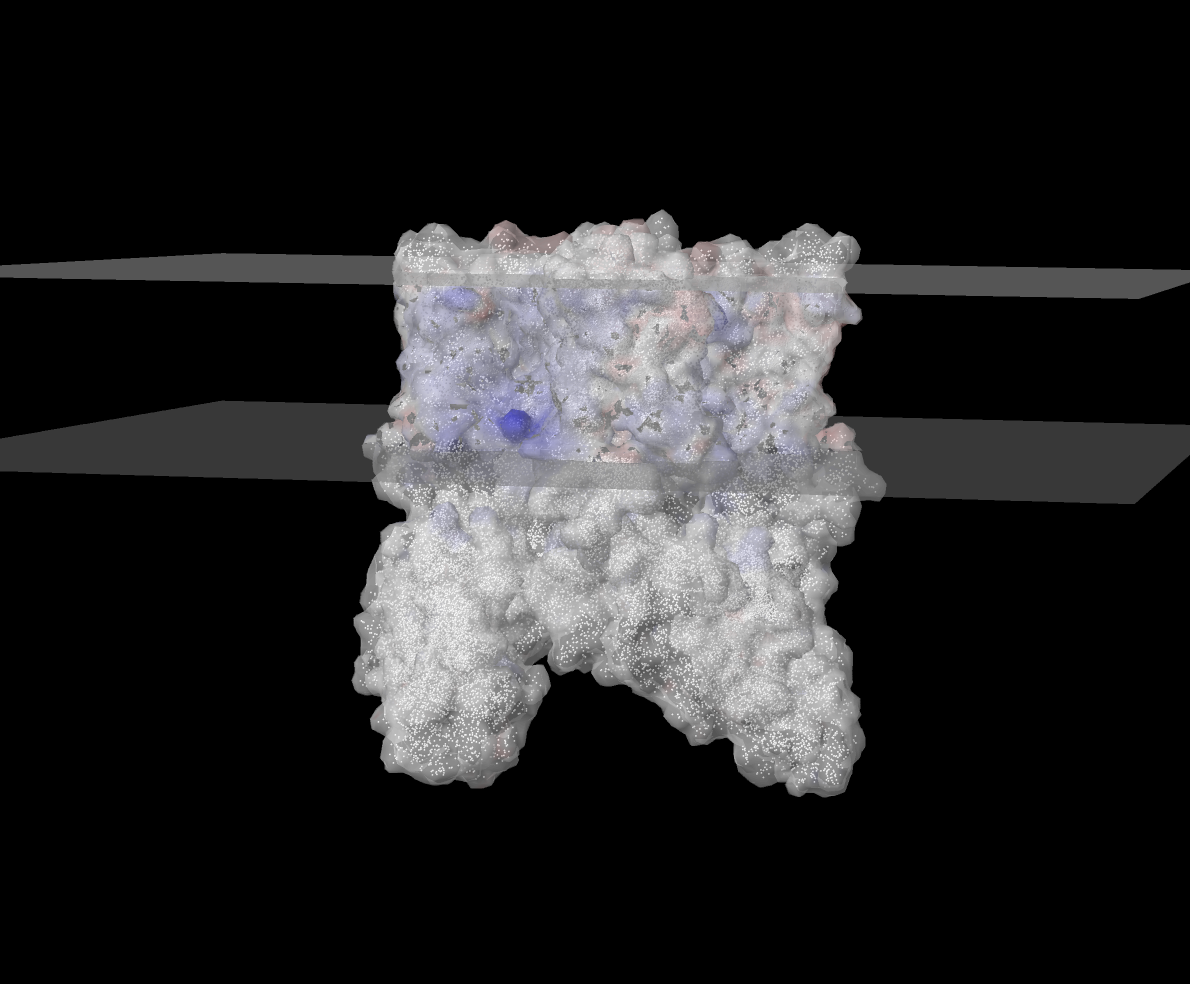
\includegraphics[scale=0.1]{./Figures/TRPV1_003.png}
		\end{minipage}%
		\begin{minipage}{0.4\slidewidth}
			\hspace*{10pt}
			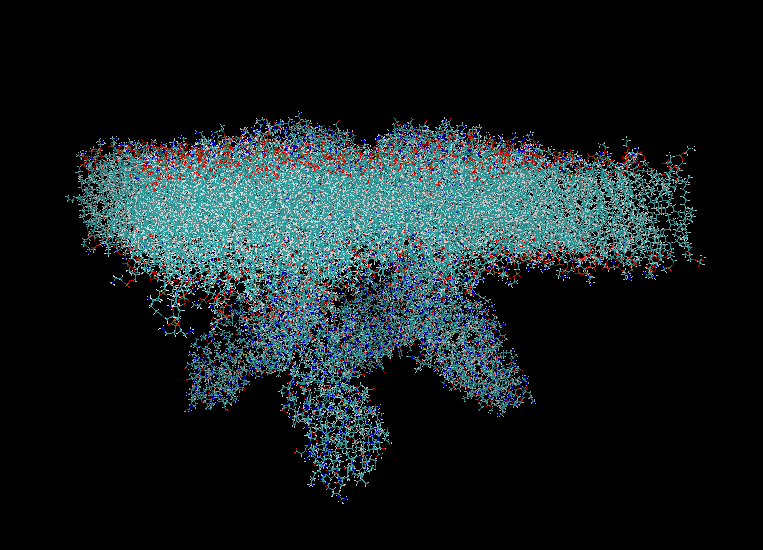
\includegraphics[scale=0.18]{./Figures/TRPV1_1.png}
		\end{minipage}
	\end{figure}
\end{frame}

\begin{frame}{Métodos numéricos, análisis continuo}
	\begin{figure}
		\begin{minipage}{0.4\slidewidth}
				{\Large\textbf{Diferencias Finitas}}\\[0.5cm]
		\end{minipage}%
		\begin{minipage}{0.4\slidewidth}
			{\Large \textbf{Elementos Finitos}}\\[0.5cm]
		\end{minipage}
	\end{figure}
\end{frame}

\begin{frame}{Boundary Element Method}
	\begin{figure}
		\begin{minipage}{0.8\slidewidth}
			\Large{Ventajas y desventajas de \textbf{BEM} como método}
		\end{minipage}
		\vspace{-1cm}
		\begin{minipage}{0.4\slidewidth}
			\input{./Figures/BEM_scheme.eps_tex}
		\end{minipage}
	\end{figure}
\end{frame}

\begin{frame}{Objetivos del trabajo}
	\begin{figure}
		\begin{minipage}{0.4\slidewidth}
			\begin{itemize}
				\item[$\bullet$] Ec. de Green con método de imágenes
				\item[$\bullet$] Calculo de energías de solvatación
			\end{itemize}
		\end{minipage}%
		\vspace{1cm}
		\begin{minipage}{0.4\slidewidth}
			\begin{itemize}
				\item[$\bullet$] Velocidad de cálculo rápida
				\item[$\bullet$] Implementación en programa
			\end{itemize}
		\end{minipage}
%		\vspace{-1cm}
		\begin{minipage}{0.55\slidewidth}
			\input{./Figures/Fig_Intro.eps_tex}
		\end{minipage}
		\vspace{-0.8cm}
	\end{figure}
\end{frame}

\section{Teoría}
	\begin{frame}{Ley de Gauss}
		\begin{equation*}
			\nabla\cdot\mathbf{E} = \frac{\rho}{\varepsilon}
		\end{equation*}
	\end{frame}



\end{document}